\chapter{Visitor}

E' un pattern comportamentale che consente di definire una nuova operazione senza modificare le classi degli oggetti su cui opera. 

Questo pattern è utile quando si ha una gerarchia di classi e si desidera eseguire diverse operazioni su di esse senza dover aggiungere nuovi metodi a ciascuna classe.

Le operazioni variano a seconda del tipo di classe concreta.

\section{Funzionamento}

Avremo un'interfaccia comune, AbstractVisitor, che definisce metodi del tipo visitXXX per ogni tipo \textbf{concreto} della struttura e le sottoclassi concrete che 
la estenderanno (implementeranno tutti i visitXXX).

Nella classe base/interfaccia della gerarchia aggiungiamo il metodo accept(...) che prende in input un AbstractVisitor e le classi concrete della gerarchia 
implementeranno questo metodo chiamando il corrispettivo metodo visitXXX passando se stesso come input.

Questo pattern sopperisce alla mancanza del \textbf{double dispatch}  (overloading dinamico).

Supponiamo di prendere in considerazione l'esempio dell'esercitazione Expression.

Quindi avremo la nostra interfaccia ExpressionVisitor con due metodi, visitConstant e visitSum che prendono in input, rispettivamente, un Constant ed un Sum e una sua 
implementazione concreta, ParenthesisRepresentationVisitor che la implementa. 

Nell'interfaccia Expression avremo il metodo accept(...) che prende in input ExpressionVisitor ed infine avremo le classi Constant e Sum che implementeranno accept(...) 
chiamando rispettivamente visitConstant e visitSum.

\section{Double dispatch}

Supponiamo di avere il seguente test

\begin{lstlisting}
@Test
public void testReprImproved() {
    ExpressionVisitor r = new ParenthesisRepresentationVisitor();
    Expression exp = new Sum(
                        new Constant(10),
                        new Constant(5)
                        );
    assertEquals("(10 + 5)", exp.accept(r));
}
\end{lstlisting}

Quando chiamiamo exp.accept(r), exp, staticamente, è di tipo Expression ma a runtime è di tipo Sum e quindi, per il binding dinamico, viene chiamato visitSum.

VisitSum, staticamente, prende in input un oggetto di tipo ExpressionVisitor che, a runtime, è di tipo ParenthesisRepresentationVisitor, quindi per il binding dinamico, 
viene chiamato ParenthesisRepVisitor.visitSum.

Ecco perchè double dispatch, ovvero abbiamo usato due volte il meccanismo del binding dinamico.

\section{Collaborazioni}

\begin{figure}[H]
  \centering
  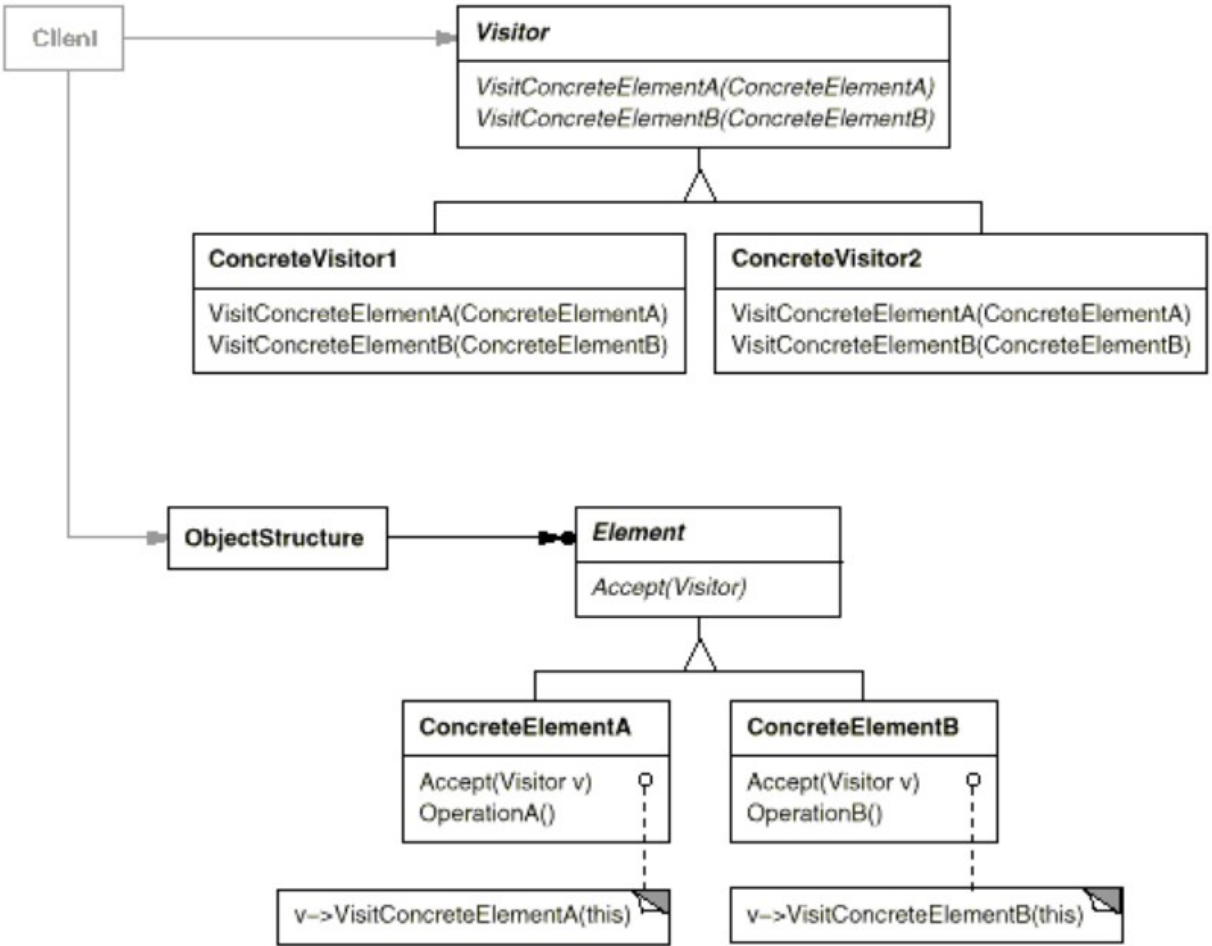
\includegraphics[width=8cm]{../../immagini/visitor/struttura_visitor}
\end{figure}

Un client crea un ConcreteVisitor e visita la struttura a oggetti.

Quando un elemento viene visitato chiama il metodo del visitor che corrisponde alla sua classe, passando se stesso come argomento, in questo modo il visitor può 
accedere allo stato dell’oggetto, se necessario

Aggiungere una nuova classe alla gerarchia, come Multipliction, comporterà aggiungere un nuovo metodo visitXXX, in ExpressionVisitor, che prenderà in input 
Multipliction ed implentare accept(...) in Multipliction.

L'aggiunta di un nuovo metodo in ExpressionVisitor, comporterà ad errori di compilazione nei visitor concreti, quindi occorrerà implementarli.

\section{Varianti Visitor}

Supponiamo di voler rimuovere il metodo eval() da Expression e di implementare la valutazione di un espressione tramite il EvalVisitor, tale che 
EvalVisitor$<:$ExpressionVisitor.

\subsection{Visitor generico}

Dall'esempio precendete, noi sappiamo che in ExpressionVisitor i metodi visitXXX ritornano una stringa, ma a noi servirebbe che i metodi visitXXX di EvalVisitor 
ritornino un integer, quindi rendiamo ExpressionVisitor generico e, a sua volta, i metodi visitXXX e accept sono generici.

Andremo a specificare l'argomento di tipo solamente quando andremo ad implementare Expression, ParenthesisRepresentationVisitor e EvalVisitor e nei test, in quanto non 
possiamo instanziare in tipo generico, instanziamo direttamente il visitor concreto.

\subsection{Visitor void}

I metodi visitXXX e accept sono void e per questo motivo ogni visitor concreto si deve mantere uno stato, che viene usato per accumulare i risultati durante la visita, 
ed infine fornire un metodo per ottenere il risultato finale di tutta la vista.

\subsection{Coseguenze}

Affinchè i visitor possano agire sugli elementi, l'interfaccia degli elementi deve fornire operazioni pubbliche di accesso e questo compromette l'incapsulamento.

E' facile aggiungere nuove operazioni, basta aggiungere un visitor completo.

E' difficile aggiungere un nuovo elemento da visitare, bisogna definire un nuovo metodo in visitor che poi dovrà essere implementato dalle classi concrete e il nuovo 
elemento da visitare deve implementare accept.

\medskip
\textbf{N.B.} Quando aggiungiamo il metodo visitXXX per la nuova classe da visitare al Visitor, i visitor concreti non compileranno più fino a quando non 
implementeremo il nuovo visitXXX in ogni visitor concreto.
\medskip

Per questo motivo, il visitor andrebbe usato quando la gerarchia degli oggetti è \textit{stabile}.

Una soluzione a questo, potrebbe essere quella di fornire un'implementazione dei metodi visitXXX in una classe astratta che implementa Visitor, cosicchè i client che 
implementeranno Visitor, estenderanno la classe astratta e ridefiniranno i metodi di loro interesse (questo però è un altro pattern).

Simulando il binding dinamico, facciamo a meno di instanceof e downcast.

Inoltre, se il linguaggio permettesse l'overloading dinamico, allora non ci sarebbe bisogno del metodo accept nelle classi da visitare ma comunque, quest'ultime, 
dovrebbero sempre fornire punti di accesso alla classe.